\documentclass[a4paper]{report}
\usepackage{setspace}

\pagestyle{plain}
\usepackage{amssymb}
\usepackage{graphicx}
\usepackage{color}
\usepackage{amsfonts}
\usepackage{latexsym}
\usepackage{amsmath}
\usepackage[toc,page]{appendix}
\setcounter{tocdepth}{1}
\usepackage{pdfpages}
\usepackage{todonotes}
\usepackage{hyperref}
\hypersetup{
    colorlinks,
    citecolor=black,
    filecolor=black,
    linkcolor=black,
    urlcolor=black
}

\usepackage[authoryear]{natbib}
\usepackage{algorithm}
\usepackage{algpseudocode}

% \usepackage{caption}
\usepackage{subcaption}
\usepackage{float}
\usepackage{lipsum}
\usepackage[a4paper, margin = 3cm, bottom = 2.5cm]{geometry}

\newtheorem{theorem}{THEOREM}
\newtheorem{lemma}[theorem]{LEMMA}
\newtheorem{corollary}[theorem]{COROLLARY}
\newtheorem{proposition}[theorem]{PROPOSITION}
\newtheorem{remark}[theorem]{REMARK}
\newtheorem{definition}[theorem]{DEFINITION}
\newtheorem{fact}[theorem]{FACT}

\newcommand{\nats}{\mbox{\( \mathbb N \)}}
\newcommand{\rat}{\mbox{\(\mathbb Q\)}}
\newcommand{\rats}{\mbox{\(\mathbb Q\)}}
\newcommand{\reals}{\mbox{\(\mathbb R\)}}
\newcommand{\ints}{\mbox{\(\mathbb Z\)}}

%%%%%%%%%%%%%%%%%%%%%%%%%%

% ========================================
% Title Page
% ========================================
\title{{\vspace{-14em} 
\includegraphics[scale=0.4]{Logos/ucl_logo.png}}\\
{{\vspace{2em} \Huge Beyond the Circle: Deforming Contours in Inverse Z-Transform}}\\
{\large Final Year Project Report}\\
}
\date{Submission date: \today}
\author{Roman Ryan Karim\thanks{
{\bf Disclaimer:}
This report is submitted as part requirement for the MEng degree in Mathematical Computation at UCL. It is substantially the result of my own work except where explicitly indicated in the text. The report may be freely copied and distributed provided the source is explicitly acknowledged.}
\\ \\ Dr Carolyn Phelan
\\ \\ \\ \\ Department of Computer Science
\\ University College London
\\ \\
}


% ========================================
% Report
% ========================================
\begin{document}
 
\onehalfspacing
\maketitle
\begin{abstract}

\end{abstract}

% ========================================
% Contents
% ========================================
\tableofcontents
\setcounter{page}{1}

% ========================================
% TODO List
% ========================================
\listoftodos

% ========================================
% Introduction
% ========================================
\chapter{Introduction}
\section{Motivation}

\section{Aims and Objectives}

\section{Overview}

% ========================================
% Background
% ========================================
\chapter{Background}

In Chapter 2, we establish a foundational understanding of the topic in hand. This section is designed to be self-contained, providing essential background for all readers, while references are included for those seeking deeper exploration. The focus is on making complex concepts accessible, ensuring a broad audience can engage with the material.

``By definition, a complex number $z$ is an ordered pair ($x, y$) of real numbers $x$ and $y$, written $z = (x, y)$" \citep{kreyszig2010advanced}. In practice, complex numbers are written in the form $z = x + iy$, where $x$ and $y$ are real numbers and $i$ is the imaginary unit. The set of complex numbers is denoted by $\mathbb{C}$.

\section{The \texorpdfstring{$\mathcal{Z}$}{Lg}-Transform}

The $z$-transform is a transformation of a real or complex time function $x(n)$, often used for analyzing discrete-time signals and systems. It is a generalization of the discrete-time Fourier transform (DTFT) that extends the analysis to the complex plane. The Z-transform is formally defined as:

\begin{equation}\label{bilateral_z-transform}
X(z) = \mathcal{Z}_{n \rightarrow z}[x(n)] = \sum^{\infty}_{n = -\infty} x(n)z^{-n}
\end{equation}

For a complete description of $z$ in the complex plane, we tend to its polar form $z = re^{i\theta}$, where $r$ represents the magnitude of $z$ and $\theta$ represents the angle of $z$ with respect to the positive real axis.

In the analysis of causal systems - systems for which a time origin is defined and is illogical to consider signal values for negative time - the unilateral $z$-transform is used. Unlike the bilateral $z$ transform in Equation (\ref{bilateral_z-transform}), we sum from zero to positive infinity yielding

\begin{equation}\label{unilateral_z-transform}
X(z) = \mathcal{Z}_{n \rightarrow z}[x(n)] = \sum^{\infty}_{n = 0} x(n)z^{-n}
\end{equation}

The region within the complex $z$-plane where the $z$-transform converges is known as the Region of Convergence (ROC). The ROC is defined for the set of values of $z$ for which the $z$-transform is absolutely summable

\begin{equation}\label{roc}
\textbf{ROC} = \Biggl\{ z : \sum^{\infty}_{n = 0} |x(n)z^{-n}| < \infty \Biggr\}
\end{equation}

For causal sequences, the ROC is typically the exterior of the outermost pole in the $Z$-plane, denoted as $|z| > a$. If we say that $z_1$ converges, then $z_1$ exists within the ROC. Thus, all $z$ such that $|z|$ For a stable system, the ROC must include the unit circle, $|z| = 1$, implying that all poles must lie within the unit circle \citep{LovelessGuido2021}.

\subsection{Relation to the Fourier Transform}
It is useful to note the relationship between the $z$-transform and the Fourier transform. Taking the Fourier transform of a sampled function $x(t)$ results in:

\begin{flalign}
&& \mathcal{F}\bigg[x(t) \sum^{\infty}_{n = -\infty} \delta(t - n \Delta t)\bigg] &= \int^{\infty}_{-\infty} x(t) \sum_{n = - \infty}^{\infty} \delta (t - n\Delta t)e^{-i \omega t} dt && \\
&& &= \sum_{n = - \infty}^{\infty} \int^{\infty}_{-\infty} x(t) \delta (t - n\Delta t)e^{-i \omega t} dt && \\
&& &= \sum^{\infty}_{n=-\infty} x(n \Delta t)e^{-i \omega nt} &&
\end{flalign}

where we make use of the sifting property of the delta function. If we normalise the sampling interval to 1, we get

\begin{equation}\label{dtft}
\sum^{\infty}_{n = - \infty} x(n)e^{-i n \omega}
\end{equation}

This is the discrete-time Fourier transform (DTFT) of the sequence $x(n)$. The sequence $x(n)$ is sampled at discrete-time intervals $t_n = n \triangle t$, where the sampling interval $\triangle t$ is the time between consecutive samples and the time index $n$ numbers the samples. The DTFT is a periodic function of $\omega$ with period $2\pi$, and its existence relies on the absolute summability of the sequence $x(n)$:

\begin{equation}
\sum^{\infty}_{n = -\infty} |x(n)| < \infty
\end{equation}

The Z-transform generalizes the discrete-time Fourier transform to the complex plane, not just the unit circle where $r = 1$. By setting $z = e^{i\omega}$ in the Z-transform, we obtain the DTFT (\ref{dtft}).

\section{Probability Discrete Functions}\label{pgfs}

\section{The Inverse \texorpdfstring{$\mathcal{Z}$}{Lg}-Transform}

The inverse $Z$-transform aims to find the $n$-th value of the sequence $x(n)$ given the $Z$-transform $X(z)$. This is commonly defined as a Cauchy integral around a contour $C$ in the complex plane. The contour $C$ is a counter-clockwise closed path that encloses the region of convergence (ROC). The inverse $Z$-transform is formally given by

\begin{equation}\label{inverse_z-transform}
	x(n) = \mathcal{Z}^{-1}_{z \rightarrow n}[X(z)] = \frac{1}{2\pi i} \oint_C X(z)z^{n-1}dz
\end{equation}

In real-world applications, we often require numerical approximation due to computational challenges posed by the Cauchy integral formula. Such approximations enable the effective analysis and processing of complex signals within various technological and financial systems.

\subsection{Abate and Whitt 1992}
The numerical approximation formula offered by \citet{AbateWhitt1992a, AbateWhitt1992b} is based on a Fourier series catering to the inversion of probability generating functions as elucidated in Section \ref{pgfs}. The format is conducive to queuing theory and other probabilistic models where the $Z$-transform is defined as $q = 1 / z$. The authors approximate the inversion using a trapezoidal rule for numerical integration over a complex contour given by

\begin{equation}\label{aw_inversion_original}
	x(n) \approx \frac{1}{2nr^n} \biggr( X(r) + 2\sum^{n-1}_{k = 1} (-1)^k \mathrm{Re}\bigg( X(re^{\frac{ik\pi}{n}})\bigg) + (-1)^nX(-r) \biggl)
\end{equation}

The parameter $r$ is used to control the error; setting $r = 10^{-\lambda / 2n}$ yields an accuracy bound of $10^{-\lambda}$. The authors leverage the inherent symmetry within the complex plane to enhance computational efficiency by exploiting the complex conjugate symmetry of $X(z)$; each term $X(re^{\frac{ik\pi}{n}})$ in the upper half has a mirror image in the lower half. The computational load is thus halved by \textit{folding} the problem in this manner.

Given the nature of this project, we may find it easier to use the following definition, where we set $z = 1 / q$, to approximate (\ref{inverse_z-transform}).

\begin{equation}\label{aw_inversion}
	x(n) \approx \frac{1}{2nr^n} \biggr( X(\frac{1}{r}) + 2\sum^{n-1}_{k = 1} (-1)^k \text{Re}\bigg( X\big(\frac{1}{re^{\frac{ik\pi}{n}}}\big)\bigg) + (-1)^nX(-\frac{1}{r}) \biggl)
\end{equation}
\todo[inline]{talk about the Nyquist-Shannon sampling theorem? - number of points must be double to avoid aliasing}

\subsection{Cavers 1978}

\subsection{Series acceleration techniques}

\section{Discrete Pricing Options}

\subsection{Lookback and Barrier Options}

\section{Optimization Techniques}
In the context of computational mathematics, optimizations techniques are used to identify the optimal or a sufficiently effective solution to a problem within a given set of constraints. The goal is to minimize or maximize a specific objective function by systematically choosing the values of the variables. The objective function is often referred to as the \textit{cost function} or \textit{loss function} and the variables are referred to as \textit{parameters}. The optimization problem can be formulated as

\begin{equation}\label{optimization_problem}
	\text{minimize } f(x) \text{ subject to } x \in \Omega
\end{equation}

where $f(x)$ is the objective function and $\Omega$ is the feasible region defined by the constraints of the problem.

Gradient descent is one of the most popular algorithms for parameter optimization with success in Deep Learning and Neural Networks employing variants of the algorithm \citep{lu2017improved, zhang2019gradient, zeebaree2019trainable}. The adaptability to diverse problem domains \citep{YingjieYugiHaibin2023SGD} parallels our use case, where gradient descent is applied outside traditional deep learning to optimize parameters of a mathematical function \citep{GradientBasedOpt2022}. This reinforces the potential of gradient descent algorithms in broader computational mathematics, affirming its efficacy in finding optimal solutions in complex optimization landscapes.

\subsection{Gradient Descent}
Gradient descent iteratively converges to a local minimum of a function by moving in the direction of the steepest descent, as defined by the negative gradient. This method is expressed mathematically as

\begin{equation}\label{GD}
    x_{k+1} = x_k - \alpha_k \nabla f(x_k)
\end{equation}

where $x_k$ is the parameter vector at iteration $k$, $\alpha_k$ is the learning rate, and $\nabla f(k)$ represents the gradient of the function at $x_k$. The selection of $\alpha_k$ is crucial as it determines the size of the step taken towards the minimum; too large can overshoot the minimum, too small can result in a long convergence time. The process repeats until a predetermined termination criterion is met, typically when the change in the value of $f$ falls below a threshold. This iterative process is showcased in the pseudocode below:

\begin{algorithm}
\caption{Gradient Descent}
\begin{algorithmic}[1]
\State Initialize \( x_0 \), set \( k = 0 \)
\While{termination conditions not met}
    \State Compute gradient \( \nabla f(x_k) \)
    \State Choose a suitable step size \( \alpha_k \)
    \State Update \( x_{k+1} = x_k - \alpha_k \nabla f(x_k) \)
    \State \( k = k + 1 \)
\EndWhile
\end{algorithmic}
\end{algorithm}

\subsubsection{Stochastic Gradient Descent}

However, classic Gradient Descent faces limitations, including susceptibility to local minima and potential for overshooting or long convergence times. Stochastic Gradient Descent (SGD) addresses these issues by introducing variability in the optimization process. It modifies (\ref{GD}) to use a randomly selected subset of data to compute the gradient, to allow for dynamic adjustment of the learning rate and leveraging noise to escape local minima. We define the update rule to 

\begin{equation}\label{SGD}
x_{k+1} = x_k - \alpha_k \nabla f_{i_k}(x_k)	
\end{equation}
where $\nabla f_{i_k}(x_k)$ is the gradient of the cost function with respect to a random subset $i_k$. We thus avoid the pitfalls associated with a static learning rate and promotes a quicker convergence time.

% ========================================
% Experiment
% ========================================
\chapter{Experiment}

\todo[inline]{Finding different parameters to use for the experiment making use of Machine Learning techniques.}

% ========================================
% Results
% ========================================
\chapter{Results}

% ========================================
% Conclusion
% ========================================
\chapter{Conclusion}
\section{Summary}

\section{Future Work}

\section{Acknowledgements}


% ========================================
% References 
% ========================================
\addcontentsline{toc}{chapter}{References}
\bibliography{references}
\bibliographystyle{apalike}

% ========================================
% Appendix
% ========================================
\begin{appendices}

\chapter{Initial Project Plan}

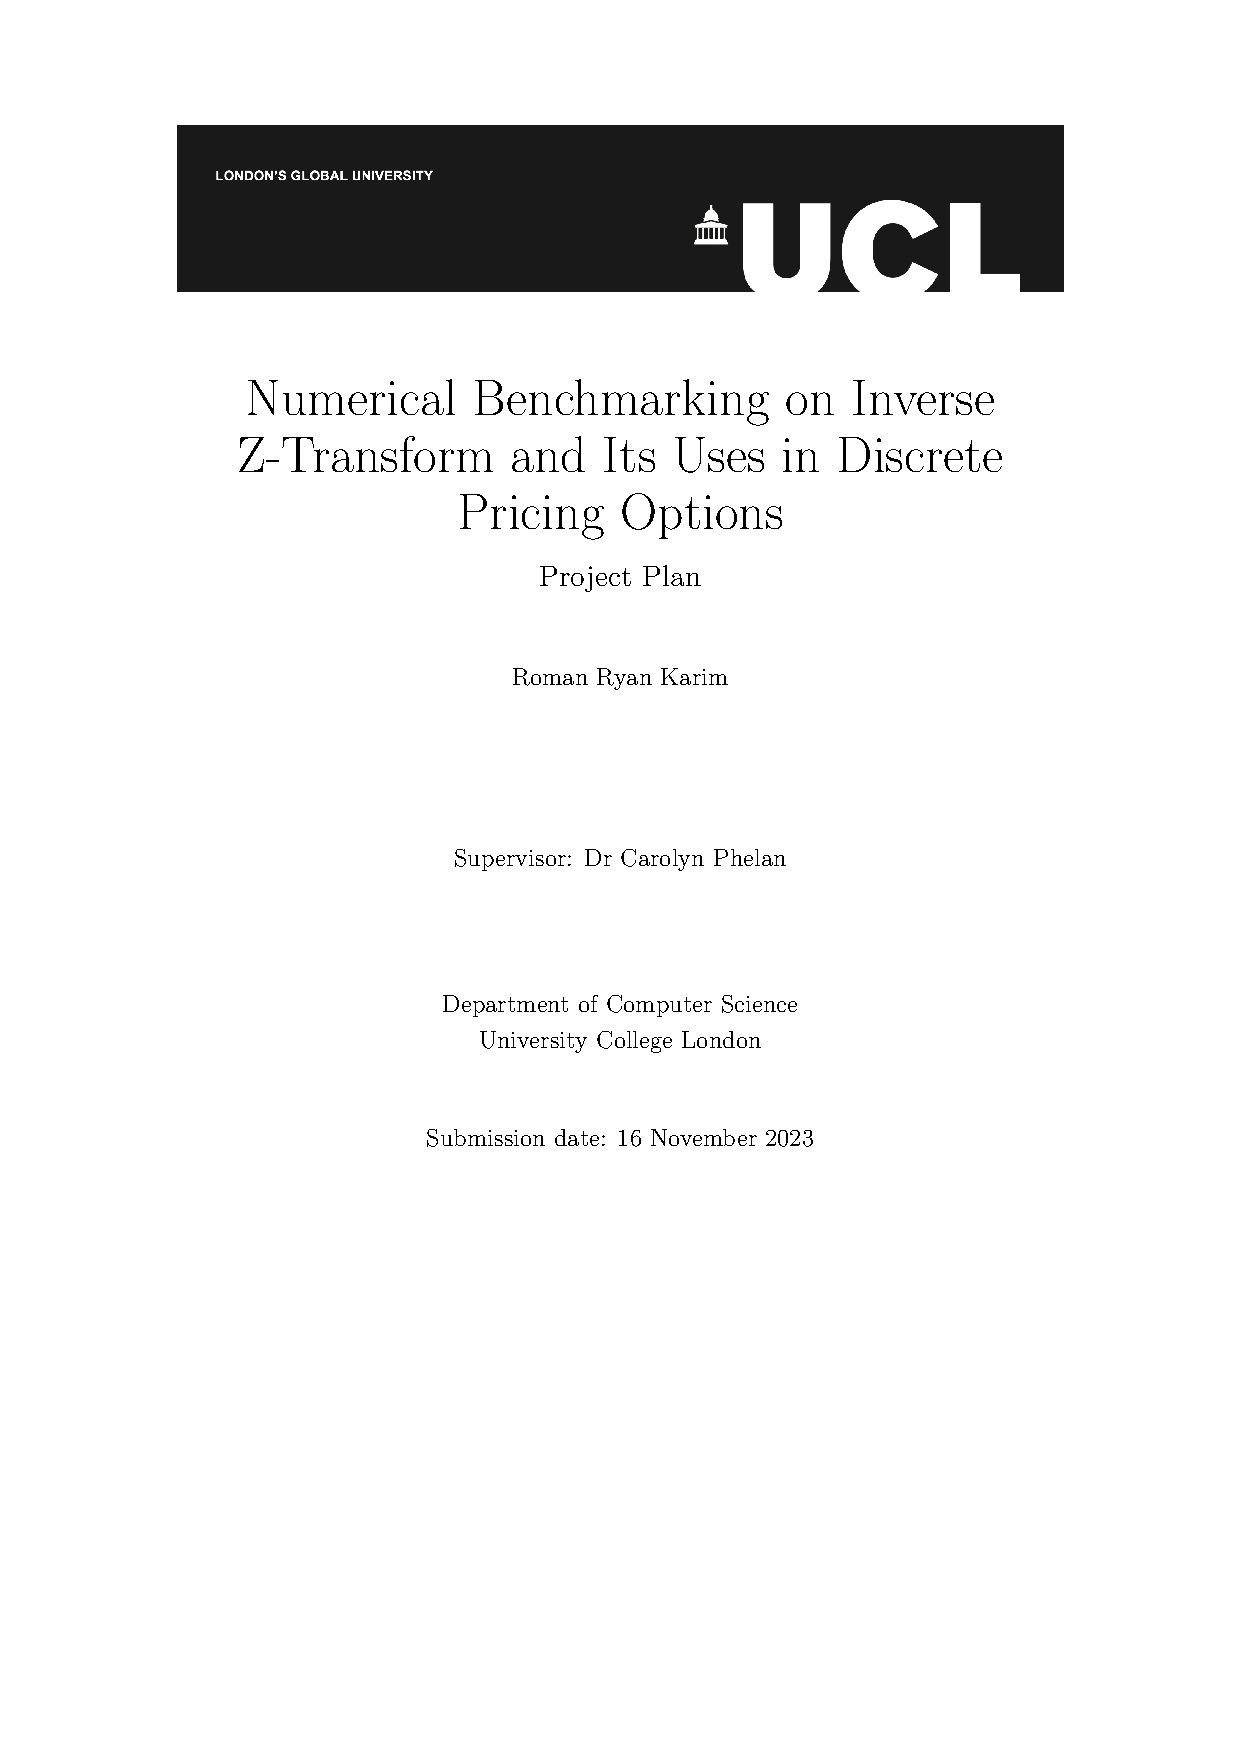
\includepdf[pages=-]{initial_project_plan.pdf}
    
\end{appendices}

\end{document}